\section{Mapping StreamIt Patterns to the Runtime Library}\label{ch:use}

There are a number of common execution patterns that can be used to run a StreamIt program (see section~\ref{ch:bg:str:exec}). To illustrate how these patterns can be mapped to the runtime library for Cell, we will refer to the FFT StreamIt benchmark as a concrete example. This program performs a 256-element fast Fourier transform. The program's stream graph consists of a single pipeline of 15 filters. Every filter in the pipeline is stateless (and hence data-parallel) and does not peek. A single complete execution of the stream graph processes a single set of 256 input elements (512 floats), producing the same number of output elements.

%% \begin{figure}[!htb]
%% \begin{center}
%% 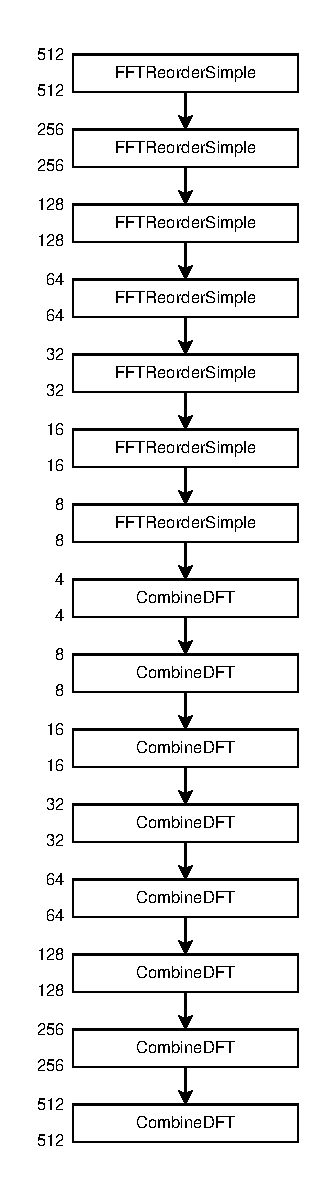
\includegraphics{figs/fftgraph}
%% \end{center}
%% \caption[Stream graph for 256-element FFT.]{Stream graph for 256-element FFT. A single execution of the stream graph pops and pushes 512 floats, since each element is a complex number whose components are interleaved on tapes.}
%% \label{fig:use:fftgraph}
%% \end{figure}

Data-parallel filters are the simplest to map to the library. The entire FFT pipeline can be fused into a single data-parallel filter that pops and pushes 512 floats per work function iteration. The fused filter can be data-parallelized over many SPEs: pseudocode to do this is illustrated in figure~\ref{fig:use:dp}. The \textsf{ext\_ppu\_spu\_ppu\_ex} library function starts an extended operation that loads the filter, allocates its buffers, and runs it for a large number of iterations.\footnote{The user still specifies all major parameters -- for example, the addresses to allocate buffers at and how many iterations each \textsf{filter\_run} command runs for.} The line containing \textsf{spulib\_poll\_while} synchronizes all SPEs; it returns only when all SPEs have finished and the callback has been run for each SPE.

\begin{figure}[!htb]
\begin{center}
\begin{tabular}{ll}
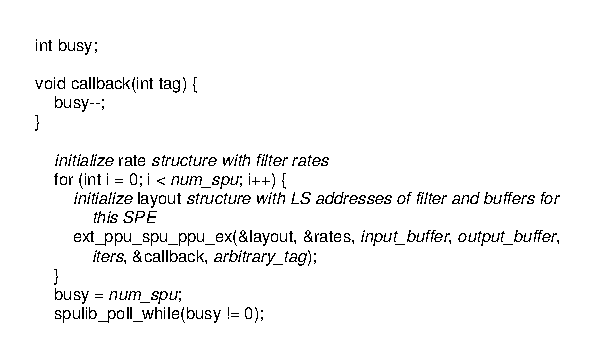
\includegraphics{figs/dpcode} & 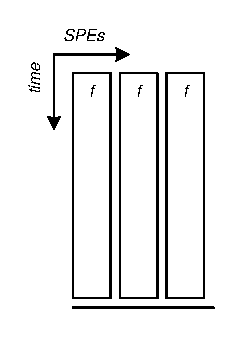
\includegraphics{figs/dp}
\end{tabular}
\end{center}
\caption[Pseudocode for running a data-parallel filter.]{Pseudocode for running a data-parallel filter. The figure on the right represents the state of each SPE as time passes. The horizontal line indicates synchronization by the PPE.}
\label{fig:use:dp}
\end{figure}

Course-grained software pipelining~\cite{asplos06} can be implemented similarly. Typically, the user will have assigned each filter in the steady state to an SPE and allocated and populated a buffer in memory for each channel. Pseudocode to execute a single iteration of the steady state is illustrated in figure~\ref{fig:use:swpipe}. Again, the line containing \textsf{spulib\_poll\_while} synchronizes all SPEs; this is necessary to ensure that sufficient input data has been produced for every filter in the next steady state iteration. For efficiency, the steady state should be sufficiently coarsened to amortize the overhead while SPEs are switching between filters and thus not performing any computation.

\begin{figure}[!htb]
\begin{center}
\begin{tabular}{ll}
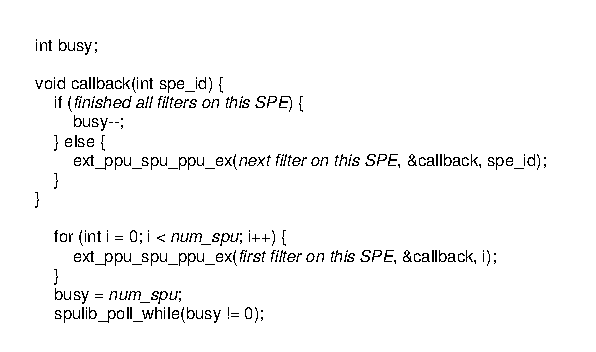
\includegraphics{figs/swpipecode} & 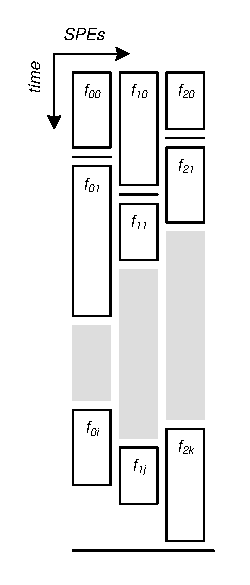
\includegraphics{figs/swpipe}
\end{tabular}
\end{center}
\caption[Pseudocode for running a course-grained software pipeline.]{Pseudocode for running a course-grained software pipeline. The figure on the right represents the state of each SPE as time passes. Horizontal lines indicate synchronization by the PPE.}
\label{fig:use:swpipe}
\end{figure}

Both patterns presented so far involve no direct SPE--SPE communication. An alternative implementation for FFT partially fuses the 15 filters in the StreamIt pipeline into a number of library filters, which are simultaneously run on different SPEs. These SPEs can transfer data between local stores directly, taking advantage of Cell's on-chip communication network and avoiding the extra latency to memory, as well as preventing memory from possibly becoming a bottleneck. Pseudocode to do this is illustrated in figure~\ref{fig:use:spepipecode}.

%% \begin{figure}[!htb]
%% \begin{center}
%% 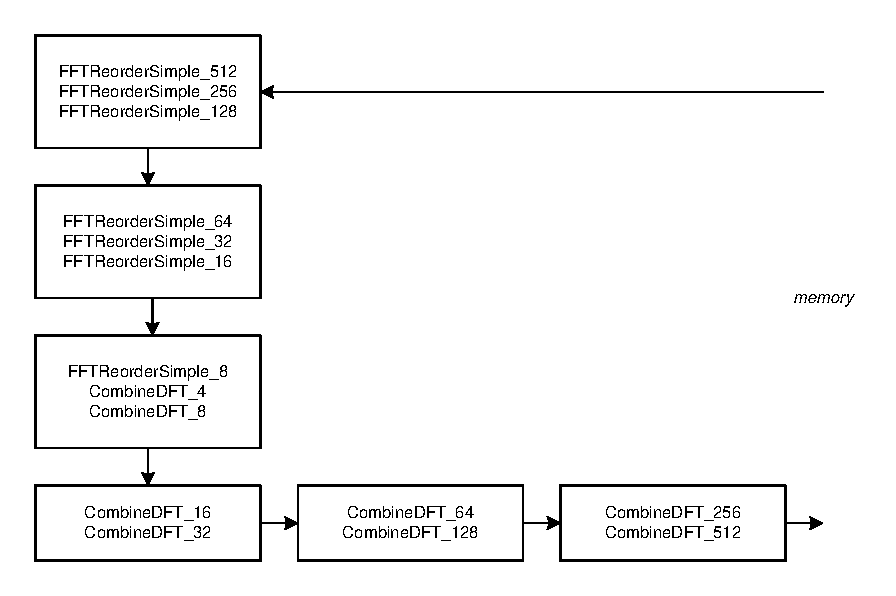
\includegraphics{figs/spepipe}
%% \end{center}
%% \caption{Pipelining FFT over six SPEs.}
%% \label{fig:use:spepipe}
%% \end{figure}

\begin{figure}[!htb]
\begin{center}
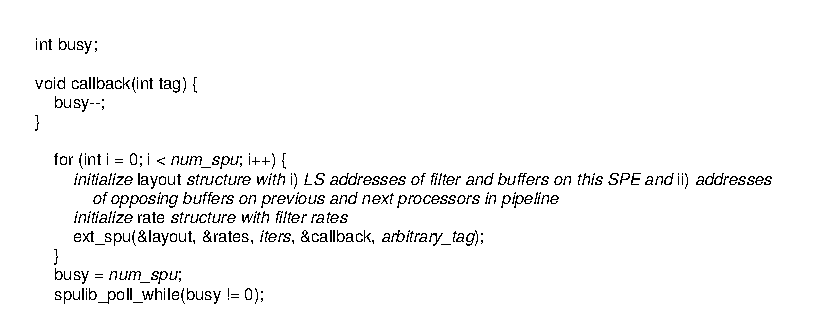
\includegraphics{figs/spepipecode}
\end{center}
\caption{Pseudocode for setting up an SPE--SPE pipeline.}
\label{fig:use:spepipecode}
\end{figure}

More complex scheduling choices require the user to provide more complex callback functions. For example, the communication overhead of loading a new filter onto an SPE can be hidden if the load is performed while the old filter is still running its last iterations.

The library allows the user to treat filters as individual schedulable entities, instead of having to consider complex lower-level operations. The pseudocode in figure~\ref{fig:use:dp} can be compared to the SPE code required to execute the same pattern (a single fused data-parallel filter) without using the library, illustrated in figure~\ref{fig:use:handcode}.

\begin{figure}[!htb]
\begin{center}
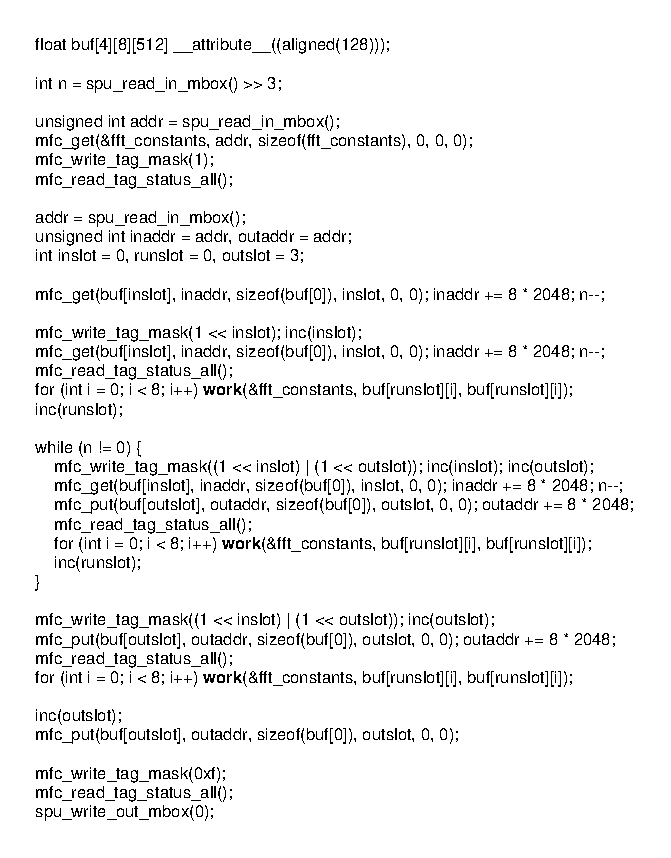
\includegraphics{figs/handcode}
\end{center}
\caption[SPE code for hand-coded implementation of data-parallel fused FFT.]{SPE code for hand-coded implementation of data-parallel fused FFT. The three bolded calls to \textsf{work} actually run the fused work function; the rest of the code performs double-buffered data transfers.}
\label{fig:use:handcode}
\end{figure}

This code is not overly complex, and will always be more efficient than using the library. However, this code is also specific to the filter and the execution pattern. The fused filter in FFT does not peek, and conveniently produces and consumes amounts of data that are compatible with Cell's DMA alignment requirements. The code would have to be significantly changed if a filter with slightly different rates were substituted. If multiple filters need to be run on an SPE, the code would then acquire additional logic to switch between filters. To run filters in an SPE--SPE pipeline, additional code would be needed to synchronize between SPEs. Using the library, the user does not need to deal with any of this.

\section{Splitters and Joiners}

In general, the type of fine-grained data reorganization performed by round-robin splitters and joiners cannot be directly implemented using Cell's DMA mechanism, which has strict alignment requirements. However, since the library supports filters with multiple input and/or output tapes, a compiler can simply define separate filters for each splitter and joiner. A compiler can also fuse a splitter or joiner with the upstream or downstream filter, respectively; the resulting filter has a much lower communication--computation ratio than an independent splitter or joiner.

The user can ignore duplicate splitters as long as the output of the upstream filter is buffered into memory. Because multiple PPE buffers can refer to the same data region, no duplication of data in memory is necessary. However, if the filters downstream of the splitter run on different SPEs, the same data must be copied to the local store of each SPE.
